\chapter[字符串视图]{字符串视图(String Views)}\label{ch19}
在C++17中,C++标准库引入了一个特殊的字符串类:\texttt{std::string\_view},
它能让我们像处理字符串一样处理字符序列,而不需要为它们分配内存空间。
也就是说,\texttt{std::string\_view}类型的对象只是引用一个外部的字符序列,
而不需要持有它们。因此,一个字符串视图对象可以被看作字符串序列的\emph{引用}。

\begin{figure}[htb]
    \begin{center}
        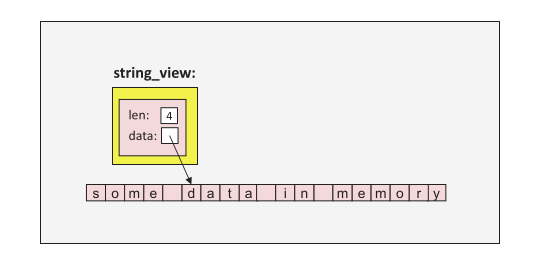
\includegraphics[scale=0.8]{../imgs/19.1.png}
        \caption{字符串视图对象}
        \label{f19.1}
    \end{center}
\end{figure}

使用字符串视图的开销很小,速度却很快(以值传递一个\texttt{string\_view}的开销总是很小)。
然而,它也有一些潜在的危险,就和原生指针一样,在使用\texttt{string\_view}时也必须
由程序员自己来保证引用的字符串序列是有效的。


\section{和\texttt{std::string}的不同之处}
和\texttt{std::string}相比,\texttt{std::string\_view}对象有以下特点:
\begin{itemize}
    \item 底层的字符序列是只读的。没有操作可以修改底层的字符。你只能赋予一个新值、
    交换值、把视图缩小为字符序列的子序列。
    \item 字符序列不保证有空字符终止。因此,字符串视图并不是一个\emph{空字符终止的字节流(NTBS)}。
    \item \texttt{data()}返回的值可能是\texttt{nullptr}。例如,当用默认构造函数初始化一个
    字符串视图之后,调用\texttt{data()}将返回\texttt{nullptr}。
    \item 没有分配器支持。
\end{itemize}
因为可能返回\texttt{nullptr},并且可能不以空字符结尾,
所以在使用\texttt{operator[]}或\texttt{data()}之前应该
总是使用\texttt{size()}获取长度
(除非你已经知道了长度)。


\section{使用字符串视图}
字符串视图有两个主要的应用:
\begin{enumerate}
    \item 你可能已经分配或者映射了字符序列或者字符串的数据,
    并且想在不分配更多内存的情况下使用这些数据。典型的例子是内存映射文件或者处理长文本的子串。
    \item 你可能想提升接收字符串为参数并以只读方式使用它们的函数/操作的性能,
    且这些函数/操作不需要结尾有空字符。

    这种情况的一种特殊形式是想以类似于\texttt{string}的API来处理字符串字面量对象:
    \begin{lstlisting}
    std::string_view hello{"hello world"};
    \end{lstlisting}
\end{enumerate}
第一个应用通常意味着只需要传递字符串视图,然而程序逻辑必须保证底层的字符序列仍然有效
(即内存映射文件不会中途取消映射)。
你也可以在任何时候使用一个字符串视图来初始化或赋值给\texttt{std::string}。

注意不要把字符串视图当作“更好的string”来使用。
这样可能导致性能问题和一些\hyperref[ch19.3.1]{运行时错误}。
请仔细的阅读下面的小节。


\section{使用字符串视图作为参数}
下面是使用字符串视图作为只读字符串的第一个例子,
这个例子定义了一个函数将传入的字符串视图作为前缀,之后打印一个集合中的元素:
\begin{lstlisting}
    #include <string_view>

    template<typename T>
    void printElems(const T& coll, std::string_view prefix = {})
    {
        for (const auto& elem : coll) {
            if (prefix.data()) {    // 排除nullptr
                std::cout << prefix << ' ';
            }
            std::cout << elem << '\n';
        }
    }
\end{lstlisting}
这里,把函数参数声明为\texttt{std::string\_view},与声明为\texttt{std::string}比较起来,
可能会减少一次分配堆内存的调用。具体的情况依赖于是否传递的是短字符串和是否使用了短字符串优化(SSO)。
例如,如果我们像下面这么声明:
\begin{lstlisting}
    template<typename T>
    void printElems(const T& coll, const std::string& prefix = {});
\end{lstlisting}
然后传递了一个字符串字面量,那么这个调用会创建一个临时的string,这将会在堆上分配一次内存,
除非使用了短字符串优化。
通过使用字符串视图,将不会分配内存,因为字符串视图只\emph{指向}字符串字面量。

注意在使用值未知的字符串视图前应该检查\texttt{data()}来排除\texttt{nullptr}。
这里为了避免写入额外的空格分隔符,必须检查\texttt{nullptr}。
值为\texttt{nullptr}的字符串视图写入到输出流时不应该写入任何字符。

另一个例子是使用字符串视图作为只读的字符串来改进\hyperref[ch15.1.1]
{\texttt{std::optional<>}章节的\texttt{asInt()}示例},
改进的方法就是把参数声明为字符串视图:\label{改进asInt}
\inputcodefile{lib/asint.cpp}
将\texttt{asInt()}的参数改为字符串视图之后需要进行很多修改。
首先,没有必要再使用\texttt{std::stoi()}来转换为整数,因为\texttt{stoi()}的参数是string,
而根据string view创建string的开销相对较高。

作为代替,我们向新的标准库函数\hyperref[ch31.2.1]{\texttt{std::from\_chars()}}传递了字符范围。
这个函数需要两个字符指针为参数,分别代表字符序列的起点和终点,并进行转换。
注意这意味着我们可以避免单独处理空字符串视图,这种情况下\texttt{data()}返回\texttt{nullptr},
\texttt{size()}返回0,因为从\texttt{nullptr}到\texttt{nullptr+0}是一个有效的空范围
(任何指针类型都支持与0相加,并且不会有任何效果)。

\texttt{std::from\_chars()}返回一个\texttt{std::from\_chars\_result}类型的结构体,
它有两个成员:一个指针\texttt{ptr}指向未被处理的第一个字符,
另一个成员\texttt{ec}的类型是\texttt{std:errc},\texttt{std::errc\{\}}代表没有错误。
因此,使用返回值中的\texttt{ec}成员初始化\texttt{ec}之后(使用了\nameref{ch1}),
下面的检查将在转换失败时返回\hyperref[nullopt]{\texttt{nullopt}}:
\begin{lstlisting}
    if (ec != std::errc{}) {
        return std::nullopt;
    }
\end{lstlisting}
使用字符串视图还可以显著\hyperref[ch22.1.2.1]{提升子字符串排序的性能}。

\subsection{字符串视图有害的一面}\label{ch19.3.1}
通常“智能对象”例如智能指针会比相应的语言特性更安全(至少不会更危险)。
因此,你可能会有一种印象:字符串视图是一种字符串的引用,应该比字符串引用更安全或者至少一样安全。
然而不幸的是,事实并不是这样的,字符串视图远比字符串引用或者智能指针更危险。
它们的行为更近似于原生字符指针。

\subsubsection{不要把临时字符串赋值给字符串视图}
考虑声明一个返回新字符串的函数:
\begin{lstlisting}
    std::string retString();
\end{lstlisting}
使用返回值总是安全的:
\begin{itemize}
    \item 用返回值来初始化一个string或者用\texttt{auto}声明的对象是安全的:
    \begin{lstlisting}
    std::string s1 = retString();   // 安全
    \end{lstlisting}
    \item 用返回值初始化常量string引用,只在局部使用时也是安全的。
    因为引用会延长返回值的生命周期:
    \begin{lstlisting}
    std::string& s2 = retString();  // 编译期ERROR(缺少const)

    const std::string& s3 = retString();  // s3延长了返回的string的生命周期
    std::cout << s3 << '\n';        // OK
    auto&& s4 = retString();        // s4延长了返回的string的生命周期
    std::cout << s4 << '\n';        // OK
    \end{lstlisting}
\end{itemize}
字符串视图没有这么安全,它\emph{既不}拷贝\emph{也不}延长返回值的生命周期:
\begin{lstlisting}
    std::string_view sv = retString(); // sv不延长返回值的生命周期
    std::cout << sv << '\n';           // 运行时ERROR:返回值已经被销毁
\end{lstlisting}
这里,在第一条语句结束时返回的字符串已经被销毁了,所以使用指向它的字符串视图\texttt{sv}
将会导致未定义的运行时错误。

这个问题类似于如下调用:
\begin{lstlisting}
    const char* p = retString().c_str();
\end{lstlisting}
或者:
\begin{lstlisting}
    auto p = retString().c_str();
\end{lstlisting}
因此,当使用返回的字符串视图时必须非常小心:
\footnote{可以在这里找到关于这个例子的讨论:
\url{https://groups.google.com/a/isocpp.org/forum/\#!topic/std-discussion/Gj5gt5E-po8}}
\begin{lstlisting}
    // 非常危险:
    std::string_view substring(const std::string& s, std::size_t idx = 0);

    // 因为:
    auto sub = substring("very nice", 5); // 返回临时string的视图
                                          // 但是临时string已经被销毁了
    std::cout << sub << '\n';     // 运行时ERROR:临时字符串s已经被销毁
\end{lstlisting}

\subsubsection{返回值类型是字符串视图时不要返回字符串}
返回值类型是字符串视图时返回字符串是非常危险的。因此,你\emph{不应该}像下面这样写:
\begin{lstlisting}
    class Person {
        std::string name;
    public:
        ...
        std::string_view getName() const {  // 不要这么做
            return name;
        }
    };
\end{lstlisting}
这是因为,下面的代码将会产生运行时错误并导致未定义行为:
\begin{lstlisting}
    Person createPerson();
    auto n = createPerson().getName();  // OOPS:delete临时字符串
    std::cout << "name: " << n << '\n'; // 运行时错误
\end{lstlisting}
如果把\texttt{getName()}改为返回一个字符串类型的值或引用就不会有这个问题了,
因为\texttt{n}将会变为返回值的拷贝。

\subsubsection{函数模板应该使用\texttt{auto}作为返回值类型}
注意无意中把字符串作为字符串视图返回是很常见的。
例如,下面的两个函数单独看起来都很有用:
\begin{lstlisting}
    // 为字符串视图定义+,返回string:
    std::string operator+ (std::string_view sv1, std::string_view sv2) {
        return std::string(sv1) + std::string(sv2);
    }

    // 泛型连接函数
    template<typename T>
    T concat (const T& x, const T& y) {
        return x + y;
    }
\end{lstlisting}
然而,如果把它们一起使用就很容易导致运行时错误:
\begin{lstlisting}
    std::string_view hi = "hi";
    auto xy = concat(hi, hi);   // xy是std::string_view
    std::cout << xy << '\n';    // 运行时错误:指向的string已经被销毁了
\end{lstlisting}
这样的代码很可能在无意中被写出来。真正的问题在于\texttt{concat()}的返回类型。
如果你把返回类型交给编译期自动推导,上面的例子将会把\texttt{xy}初始化为\texttt{std::string}:
\begin{lstlisting}
    // 改进的泛型连接函数
    template<typename T>
    auto concat (const T& x, const T& y) {
        return x + y;
    }
\end{lstlisting}

\subsubsection{不要在调用链中使用字符串视图来初始化字符串}
在一个中途或者最后需要字符串的调用链中使用字符串视图可能会适得其反。
例如,如果你定义了一个有如下构造函数的类\texttt{Person}:
\begin{lstlisting}
    class Person {
        std::string name;
    public:
        Person (std::string_view n) // 不要这样做
            : name {n} {
        }
        ...
    };
\end{lstlisting}
传递一个字符串字面量或者之后还会使用的string是没问题的:
\begin{lstlisting}
    Person p1{"Jim"};       // 没有性能开销
    std::string s = "Joe";
    Person p2{s};           // 没有性能开销
\end{lstlisting}
然而,使用move的string将会导致不必要的开销。
因为传入的string首先要隐式转换为字符串视图,
之后会再用它创建一个新的string,会再次分配内存:
\begin{lstlisting}
    Person p3{std::move(s)};  // 性能开销:move被破坏
\end{lstlisting}
不要在这里使用\texttt{std::string\_view}。以值传参然后把值move到成员里仍然是
最佳的方案(除非你想要双倍的开销):
\begin{lstlisting}
    class Person {
        std::string name;
    public:
        Person (std::string n) : name{std::move(n)} {
        }
        ...
    };
\end{lstlisting}
如果我们必须创建/初始化一个string,直接作为参数创建可以让我们在传参时享受所有可能的优化。
最后只需要简单的把参数move就行了,这个操作开销很小。

因此,如果我们使用一个返回临时字符串的辅助函数来初始化一个字符串:
\begin{lstlisting}
    std::string newName()
    {
        ...
        return std::string{...};
    }

    Person p{newName()};
\end{lstlisting}
\hyperref[ch5]{强制省略拷贝}特性将把新string的实质化过程推迟到值被传递给构造函数。
构造函数里我们有了一个叫\texttt{n}的string,这是一个有内存地址的对象
(一个\emph{广义左值(glvalue)})。之后把这个对象的值move到成员\texttt{name}里。

\subsubsection{安全使用字符串视图的总结}
总结起来就是\textbf{小心地使用\texttt{std::string\_view}},
也就是说你应该按下面这样调整你的编码风格:
\begin{itemize}
    \item 不要在那些会把参数传递给string的API中使用string view。
    \begin{itemize}
        \item 不要用string view形参来初始化string成员。
        \item 不要把string设为string view调用链的终点。
    \end{itemize}
    \item 不要返回string view。
    \begin{itemize}
        \item 除非它只是转发输入的参数,或者你可以标记它很危险,例如,通过命名来体现危险性。
    \end{itemize}
    \item \textbf{函数模板}永远不应该返回泛型参数的类型\textbf{T}。
    \begin{itemize}
        \item 作为替代,返回\texttt{auto}类型。
    \end{itemize}
    \item 永远不要用返回值来初始化string view。
    \item \textbf{不要}把返回泛型类型的函数模板的返回值赋给\textbf{\texttt{auto}}。
    \begin{itemize}
        \item 这意味着AAA(\emph{总是auto(Almost Always Auto)})原则不适用于string view。
    \end{itemize}
\end{itemize}
如果因为这些规则太过复杂或者太困难而不能遵守,那就完全不要
使用\texttt{std::string\_view}(除非你知道自己在做什么)。


\section{字符串视图类型和操作}
这一节详细描述字符串视图类型和操作

\subsection{字符串视图的具体类型}
在头文件\texttt{<string\_view>}中,C++标准库为\texttt{basic\_string\_view<>}提供了很多
特化版本:
\begin{itemize}
    \item 类\texttt{std::string\_view}是预定义的字符类型为\texttt{char}的特化模板:
    \begin{lstlisting}
    namespace std {
        using string_view = basic_string_view<char>;
    }
    \end{lstlisting}
    \item 对于使用宽字符集,例如Unicode或者某些亚洲字符集的字符串,还定义了另外三个类型:
    \begin{lstlisting}
    namespace std {
        using u16string_view = basic_string_view<char16_t>;
        using u32string_view = basic_string_view<char32_t>;
        using wstring_view = basic_string_view<wchar_t>;
    }
    \end{lstlisting}
\end{itemize}
在接下来的几节中,使用哪一种字符串视图并没有任何区别。
这几种字符串视图类的用法和问题都是一样的,因为它们都有相同的接口。
因此,“string view”意味着任何string view类型:\texttt{string\_view}、
\texttt{u16string\_view}、\texttt{u32string\_view}、\texttt{wstring\_view}。
这本书中的例子通常使用类型\texttt{string\_view},因为欧洲和英美的环境是大部分软件开发的
普遍环境。

\subsection{字符串视图的操作}
表\hyperref[t19.1]{字符串视图的操作}列出了字符串视图的所有操作。
\begin{table}[htb]
    \centering
    \begin{tabular}{l|l}
        \hline
        \textbf{操作}                        & \textbf{效果}                        \\
        \hline
        \emph{构造函数}                        & 创建或拷贝一个字符串视图                       \\
        \emph{析构函数}                        & 销毁一个字符串视图                          \\
        \texttt{=}                         & 赋予新值                               \\
        \texttt{swap()}                    & 交换两个字符串视图的值                        \\
        \texttt{==、!=、<、<=、>,>=、compare()} & 比较字符串视图                            \\
        \texttt{empty()}                   & 返回字符串视图是否为空                        \\
        \texttt{size()、length()}           & 返回字符的数量                            \\
        \texttt{max\_size()}               & 返回可能的最大字符数                         \\
        \texttt{[]、at()}                   & 访问一个字符                             \\
        \texttt{front()、back()}            & 访问第一个或最后一个字符                       \\
        \texttt{<<}                        & 将值写入输出流                            \\
        \texttt{copy()}                    & 把内容拷贝或写入到字符数组                      \\
        \texttt{data()}                    & 返回\texttt{nullptr}或常量字符数组(没有空字符终止) \\
        \emph{查找函数}                        & 查找子字符串或字符                          \\
        \texttt{begin()、end()}             & 提供普通迭代器支持                          \\
        \texttt{cbegin()、cend()}           & 提供常量迭代器支持                          \\
        \texttt{rbegin()、 rend()}          & 提供反向迭代器支持                          \\
        \texttt{crbegin()、crend()}         & 提供常量反向迭代器支持                        \\
        \texttt{substr()}                  & 返回子字符串                             \\
        \texttt{remove\_prefix()}          & 移除开头的若干字符                          \\
        \texttt{remove\_suffix()}          & 移除结尾的若干字符                          \\
        \texttt{hash<>}                    & 计算哈希值的函数对象的类型                      \\
        \hline
    \end{tabular}
    \caption{字符串视图的操作}
    \label{t19.1}
\end{table}

除了\texttt{remove\_prefix}和\texttt{remove\_suffix()}之外,
所有字符串视图的操作\texttt{std::string}也都有。
然而,相应的操作的保证可能有些许不同,\texttt{data()}的返回值可能是\texttt{nullptr}
或者没有空字符终止。

\subsubsection{构造}
你可以使用很多种方法来创建字符串视图:用默认构造函数创建、用拷贝函数构造创建、从原生字符数组创建
(空字符终止或者指明长度)、从\texttt{std::string}创建或者从带有\texttt{sv}后缀的字面量创建。
然而,注意以下几点:
\begin{itemize}
    \item 默认构造函数创建的字符串视图对象调用\texttt{data()}会返回\texttt{nullptr}。
    因此,\texttt{operator[]}调用将无效。
    \begin{lstlisting}
    std::string_view sv;
    auto p = sv.data();     // 返回nullptr
    std::cout << sv[0];     // ERROR:没有有效的字符
    \end{lstlisting}
    \item 当使用空字符终止的字节流初始化字符串视图时,最终的大小是不包括\texttt{'\textbackslash 0'}在内的
    字符的数量,另外索引空字符所在的位置是无效的:
    \begin{lstlisting}
    std::string_view sv{"hello"};
    std::cout << sv;        // OK
    std::cout << sv.size(); // 5
    std::cout << sv.at(5);  // 抛出std::out_of_range异常
    std::cout << sv[5];     // 未定义行为
    std::cout << sv.data(); // OOPS:恰好sv后边还有个'\0',所以能直接输出字符指针
    \end{lstlisting}
    你可以指定传递的字符数量来把空字符初始化为字符串视图的一部分:
    \begin{lstlisting}
    std::string_view sv{"hello", 6};    // NOTE:包含'\0'的6个字符
    std::cout << sv.size();             // 6
    std::cout << sv.at(5);              // OK,打印出'\0'的值
    std::cout << sv[5];                 // OK,打印出'\0'的值
    std::cout << sv.data();             // OK
    \end{lstlisting}
    \item 为了从一个string创建一个字符串视图,有一个为\texttt{std::string}定义的隐式转换运算符。
    再强调一次,string保证在最后一个字符之后有一个空字符,字符串视图没有这个保证:
    \begin{lstlisting}
    std::string s = "hello";
    std::cout << s.size();      // 5
    std::cout << s.at(5);       // 抛出std::out_of_range异常
    std::cout << s[5];          // OK,打印出'\0'的值
    std::cout << s.data();      // OK

    std::string_view sv{s};
    std::cout << sv.size();     // 5
    std::cout << sv.at(5);      // 抛出std::out_of_range异常
    std::cout << sv[5];         // 未定义行为
    std::cout << sv.data();     // OOPS:只有当sv后有'\0'时才能正常工作
    \end{lstlisting}
    \item 因为后缀\texttt{sv}定义了字面量运算符,所以可以像下面这样创建一个字符串视图:
    \begin{lstlisting}
    using namespace std::literals;
    auto s = "hello"sv;
    \end{lstlisting}
\end{itemize}
注意\texttt{std::char\_traits}成员被改为了\texttt{constexpr},
所以你可以在编译期用一个字符串字面量初始化字符串视图:\label{编译期字符串视图}
\begin{lstlisting}
    constexpr string_view hello = "Hello World!";
\end{lstlisting}

\subsubsection{结尾的空字符}
创建字符串视图的不同方式展示了字符串视图优越的一点,理解这一点是很重要的:
一般情况下,字符串视图的值不以空字符结尾,甚至可能是\texttt{nullptr}。
因此,你应该\textbf{总是}在访问字符串视图的字符之前检查\texttt{size()}
(除非你知道了长度)。
然而,你\emph{可能}会遇到两个特殊的场景,这两个场景会让人很迷惑:
\begin{enumerate}
    \item 你可以确保字符串视图的值以空字符结尾,尽管空字符并不是值的一部分。
    当你用字符串字面量初始化字符串视图时就会遇到这种情况:
    \begin{lstlisting}
    std::string_view sv1{"hello"};      // sv1的结尾之后有一个'\0'
    \end{lstlisting}
    这里,字符串视图的状态可能让人很困惑。这种状态有明确的定义所以可以将它用作空字符结尾的
    字符序列。然而,只有当我们明确知道这个字符串视图后有一个不属于自身的空字符时才有明确的定义。
    \item 你可以确保\texttt{'\textbackslash 0'}成为字符串视图的一部分。例如:
    \begin{lstlisting}
    std::string_view sv2{"hello", 6};   // 参数6使'\0'变为值的一部分
    \end{lstlisting}
    这里,字符串视图的状态可能让人困惑:打印它的话看起来像是只有5个字符,
    但它的实际状态是持有6个字符
    (空字符成为了值的一部分,使它变得更像一个两段的字符串(视图)(binary string(view)))。
\end{enumerate}
问题在于要想确保字符串视图后有一个空字符的话,这两种方式哪一种更好。
我倾向于不要用这两种方式中的任何一种,但截止目前,C++还没有更好的实现方式。
看起来我们似乎还需要一个既保证以空字符结尾又不需要拷贝字符
的字符串视图类型(就像\texttt{std::string}一样)。
在没有更好的替代的情况下,字符串视图就只能这么用了。
事实上,我们已经可以看到很多提案建议C++标准把返回字符指针的
函数的返回类型替换为\texttt{string\_view}
(\url{https://wg21.link/P0555r0}有一个例子)。

\subsubsection{哈希}
C++标准库保证值相同的字符串和字符串视图的哈希值相同。

\subsubsection{修改字符串视图}
这里有几个修改字符串视图的操作:
\begin{itemize}
    \item 你可以赋予新值或者交换两个字符串视图的值:
    \begin{lstlisting}
    std::string_view sv1 = "hey";
    std::string_view sv2 = "world";
    sv1.swap(sv2);
    sv2 = sv1;
    \end{lstlisting}
    \item 你可以跳过开头或结尾的字符(即把起始位置后移或者把结尾位置前移)。
    \begin{lstlisting}
    std::string_view sv = "I like my kindergarten";
    sv.remove_prefix(2);
    sv.remove_suffix(8);
    std::cout << sv;    // 打印出:like my kind
    \end{lstlisting}
\end{itemize}
注意没有对\texttt{operator+}的支持。因此:
\begin{lstlisting}
    std::string_view sv1 = "hello";
    std::string_view sv2 = "world";
    auto s1 = sv1 + sv2;    // ERROR
\end{lstlisting}
两个操作数都必须是string:
\begin{lstlisting}
    auto s2 = std::string(sv1) + std::string(sv2);   // OK
\end{lstlisting}
注意字符串视图没有到string的隐式类型转换,因为这个过程需要分配内存,开销很大。
所以必须使用显式的转换。
\footnote{理论上讲,我们可以标准化一个操作来把两个字符串视图连接起来并返回新的string,
但直到目前为止还没有实现。}

\subsection{其他类型对字符串视图的支持}
理论上讲,任何需要传递字符串值的地方都可以传递字符串视图,
前提是接收者只读取值且不需要空字符结尾。

然而,到目前为止,C++标准只为大多数重要的场景添加了支持:
\begin{itemize}
    \item 使用字符串时可以联合使用字符串视图:
    \begin{itemize}
        \item 你可以从一个字符串视图创建一个string(构造函数是explicit的)。如果字符串视图
        没有值(\texttt{data()}返回\texttt{nullptr}),字符串将被初始化为空。
        \item 你可以把字符串视图用作字符串的赋值、扩展、插入、替换、比较或查找操作的参数。
        \item 存在从string到string view的隐式类型转换。
    \end{itemize}
    \item 你可以把字符串视图传给\texttt{std::quoted},它把参数用双引号括起来输出。例如:
    \begin{lstlisting}
    using namespace std::literals;

    auto s = R"(some\value)"sv;     // raw string view
    std::cout << std::quoted(s);    // 输出:"some\value"
    \end{lstlisting}
    \item 你可以使用字符串视图初始化、扩展或比较\hyperref[ch20.2.3]{文件系统路径}。
\end{itemize}
其他对字符串视图的支持,例如C++标准库中的正则表达式库的支持,仍然缺失。


\section{在API中使用字符串视图}
字符串视图开销很小并且每一个\texttt{std::string}都可以用作字符串视图。
因此,看起来好像\texttt{std::string\\
\_view}是更好的用作字符串参数的类型。然而,有一些细节很重要\ldots

首先,只有当函数按照如下约束使用参数时,使用\texttt{std::string\_view}才有意义:
\begin{itemize}
    \item 它并不需要结尾有空字符。给一个以单个\texttt{const char*}
    为参数而没有长度参数的C函数传递参数时就不属于这种情况。
    \item 它不会违反传入参数的生命周期。通常,这意味着接收函数只会在传入值的生命周期结束之前使用它。
    \item 调用者函数不应该更改底层字符的所有权(例如销毁它、改变它的值或者释放它的内存)。
    \item 它可以处理参数值为\texttt{nullptr}的情况。
\end{itemize}
注意同时有\texttt{std::string}和\texttt{std::string\_view}重载的函数可能会导致歧义:
\begin{lstlisting}
    void foo(const std::string&);
    void foo(std::string_view);

    foo("hello");   // ERROR:歧义
\end{lstlisting}
最后,记住\hyperref[ch19.3.1]{上文提到的警告}:
\begin{itemize}
    \item 不要把临时字符串赋给字符串视图。
    \footnote{译者注:此处原文是Do not assign temporary string views to strings. 应是作者笔误。}
    \item 不要返回字符串视图。
    \item 不要在调用链中使用字符串视图来初始化或重设字符串的值。
\end{itemize}
带着这些考虑,让我们来看一些使用字符串视图进行改进的例子。

\subsection{使用字符串视图代替string}
考虑下列代码:
\begin{lstlisting}
    // 带前缀输出时间点:
    void print (const std::string& prefix, const std::chrono::system_clock::time_point& tp)
    {
        // 转换为日历时间:
        auto rawtime{std::chrono::system_clock::to_time_t(tp)};
        std::string ts{std::ctime(&rawtime)};   // 注意:不是线程安全的

        ts.resize(ts.size()-1); // 跳过末尾的换行符

        std::cout << prefix << ts;
    }
\end{lstlisting}
可以被替换为下列代码:
\begin{lstlisting}
    void print (std::string_view prefix, const std::chrono::system_clock::time_point& tp)
    {
        auto rawtime{std::chrono::system_clock::to_time_t(tp)};
        std::string_view ts{std::ctime(&rawtime)};  // 注意:不是线程安全的

        ts.remove_suffix(1);    // 跳过末尾的换行符

        std::cout << prefix << ts;
    }
\end{lstlisting}
最先想到也是最简单的改进就是把只读字符串引用\texttt{prefix}换成字符串视图,
只要我们不使用会因为没有值或者没有空终止符而失败的操作就可以。
这个例子中我们只是打印字符串视图的值,这是没问题的。
如果字符串视图没有值(\texttt{data()}返回\texttt{nullptr})将不会输出任何字符。
注意字符串视图是以值传参的,因为拷贝字符串视图的开销很小。

我们也对内部\texttt{ctime()}返回的值使用了字符串视图。
然而,我们必须小心保证当我们在字符串视图中使用它时它的值还存在。
也就是说,这个值只有在下一次\texttt{ctime()}或者\texttt{asctime()}调用之前有效。
因此,在多线程环境下,这个函数将导致问题(使用string时也有一样的问题)。

如果函数返回把前缀和时间点连接起来的字符串,代码可能会像下面这样:
\begin{lstlisting}
    std::string toString (std::string_view prefix, const std::chrono::system_clock::time_point& tp)
    {
        auto rawtime{std::chrono::system_clock_to_time_t(tp)};
        std::string_view ts{std::ctime(&rawtime)};  // 注意:不是线程安全的

        ts.remove_suffix(1);    // 跳过末尾的换行符
        return std::string{prefix} + ts; // 很不幸没有两个字符串视图的+运算符
    }
\end{lstlisting}
注意我们不能简单地用\texttt{operator+}连接两个字符串视图。
我们必须把其中一个转换为\texttt{std::string}
(很不幸这个操作会分配不必要的内存)。如果字符串视图没有值
(\texttt{data()}返回\texttt{nullptr}),字符串将为空。

另一个使用字符串视图的例子是使用字符串视图和
并行算法来\hyperref[{ch22.1.2.1}]{排序子字符串}:
\begin{lstlisting}
    sort(std::execution::par, coll.begin(), coll.end(),
         // 译者注:此处原文是
         // sort(coll.begin(), coll.end(),
         // 应是作者笔误

         [] (const auto& a, const auto& b) {
             return std::string_view{a}.substr(2) < std::string_view{b}.substr(2);
         });
\end{lstlisting}
要比使用string的子字符串快得多:
\begin{lstlisting}
    sort(std::execution::par, coll.begin(), coll.end(),
         [] (const auto& a, const auto& b) {
             return a.substr(2) < b.substr(2);
         });
\end{lstlisting}
这是因为string的\texttt{substr()}函数会返回一个分配自己内存的新字符串。


\section{后记}
首个引用语义的字符串类由Jeffrey Yasskin在\url{https://wg21.link/n3334}中提出
(命名为\texttt{string\_ref})。
这个类因Jeffrey Yasskin的\url{https://wg21.link/n3921}提案
而被Library Fundamentals TS采纳。

这个类因Beman Dawes和Alisdair Meredith的\url{https://wg21.link/p0220r1}提案
而和其他组件一起被C++17标准采纳。之后为了更好的集成,Marshall Clow在
\url{https://wg21.link/p0254r2}和\url{https://wg21.link/p0403r1}中、
Nicolai Josuttis在\url{https://wg21.link/p0392r0}中添加了一些修改。

Antony Polukhin在发表于\url{https://wg21.link/p0426r1}提案中添加了对
\texttt{constexpr}的支持。

Daniel Krügler发表的\url{https://wg21.link/lwg2946}中包含了一些修复
(作为C++17的缺陷被C++20采纳)。
